
\chapter{DEPLASMAN ARTTIRMA KATSAYISI}

\label{CH3} 

Tez çalışması kapsamında sismik yalıtımlı yapıların doğrusal olmayan
hareket denklemlerinin yer ivmeleri etkisinde daha önce belirtilen
kapsam ve yöntemler dahilinde çözülebildiği MSBIS programı hazırlanmıştır.
Bu bölümde, oluşturulan algoritmanın doğrulaması yapılarak, yapısal
özellikleri açıklanmış ve ortak yalıtım düzleminde bulunan ikili yapıların,
parametrik incelenmesine dair prosedürler gösterilecektir. Daha sonra
hazırlanan çalışmaya ait sonuçlar paylaşılmıştır. Son olarak ikiden
fazla yapının ortak yalıtım düzleminde bulunması durumu için hazırlanan
örnek sistemler incelenecektir.

Numarasız denkleme örnek:

\section{Taşıyıcı Sistem Davranış Katsayısı}

Tez çalışması kapsamında sismik yalıtımlı yapıların doğrusal olmayan
hareket denklemlerinin yer ivmeleri etkisinde daha önce belirtilen
kapsam ve yöntemler dahilinde çözülebildiği MSBIS programı hazırlanmıştır.
Bu bölümde, oluşturulan algoritmanın doğrulaması yapılarak, yapısal
özellikleri açıklanmış ve ortak yalıtım düzleminde bulunan ikili yapıların,
parametrik incelenmesine dair prosedürler gösterilecektir. Daha sonra
hazırlanan çalışmaya ait sonuçlar paylaşılmıştır. Son olarak ikiden
fazla yapının ortak yalıtım düzleminde bulunması durumu için hazırlanan
örnek sistemler incelenecektir.

Numarasız denkleme örnek:
\[
\Delta=5x
\]


\section{Dayanım Fazlalığı Katsayısı}

\label{StructuralProperties} Tez çalışması kapsamında incelenen ortak
yalıtım düzleminde bulunan sismik yalıtımlı iki yapının değerlendirilmesi,
bu bölümde açıklanan yapı parametreleri kullanılarak gerçekleştirilmiştir.
Yapılar yalnızca yatay doğrusal kesme yaylarına sahip çok serbestlik
dereceli sistemlerden oluşmaktadır. Yapı elemanları, doğrusal elastik
olarak modellenmiştir. Dolayısıyla, üst yapı taşıyıcılarında deprem
yükleri altında oluşan kuvvet-yer değiştirme ilişkisinin doğrusal
elastik olduğu kabul edilmiştir. Şekil \ref{fig:structuralmodel}'de
belirtildiği gibi yalıtım düzlemi ve yapı kat döşemeleri düzlem içinde
rijit kabul edilerek tek bir kütle ile ifade edilmiştir. 
\begin{figure}[h!]
\centering{}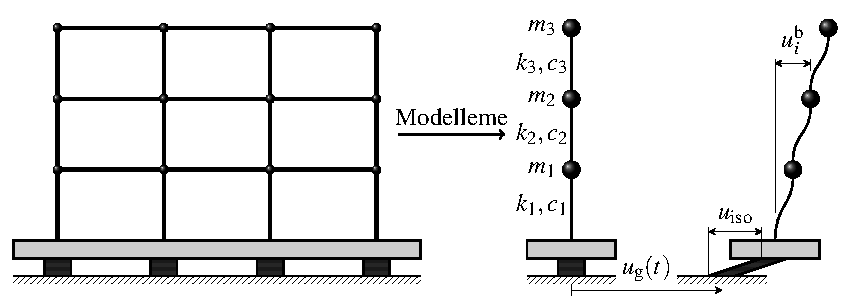
\includegraphics{TikZ/StructuralModel} \caption{\label{fig:structuralmodel}3 nolu yapıya ait analitik model ve yapının
şekil değiştirmiş hali.}
 
\end{figure}

Yapının kat rijitlikleri, tüm kolonların yatay rijitliklerinin denklem
\ref{lateralstiffness}'de verilen formüle göre belirlenerek toplanması
ile elde edilmiştir. Her bir kat için yatay rijitlik değeri, toplam
16 adet 60 $\times$ 60 cm boyutlarında betonarme kolonların yatay
rijitlikleri toplamına eşit olarak alınmıştır. Tüm yapı ve katlar
için kat yüksekliği h=4m olarak belirlenmiştir. Betonarme elastisite
modulü $E_{\text{c}}=32000\text{ MPa}$ olarak kabul edilmiştir. 
\begin{equation}
\sum\limits _{i=1}^{n}k_{i}=\dfrac{12E_{\text{c}}I}{h^{3}}\label{lateralstiffness}
\end{equation}
Burada, $k$ her bir kolona ait yatay rijitliği, $E_{\text{c}}$ betonarme
elastisite modulünü, $I$ atalet momentini, h kat yüksekliğini ve
n bir katta bulunan kolon adedini ifade etmektedir. Sismik yalıtım
sistemi ise tüm izolatörlerin yapısal özelliklerinin toplamı ile ifade
edilen doğrusal olmayan yatay kesme yayı ile tanımlanmıştır. Ayrıca
sismik yalıtımlı yapının sahip olduğu sönüm, izolatörlerin doğrusal
olmayan kesme yaylarında sönümlediği enerji ve üst yapının sahip olduğu
Rayleigh sönümü olmak üzere ayrıklaştırılmıştır. Yapısal sönüm modellerine
ait detaylar Bölüm detaylı olarak açıklanmıştır.

\section{Süneklik Azaltma Katsayısı}

sadsadasdasdaşkms alsdöaşsd 

\begin{table}[h]
\centering{}\caption{\label{structures2}Çalışma kapsamında incelenen sistemlerin tabanı
ankastre olması durumu için hesaplanan yapısal özellikleri.}
\begin{tabular}{ccccc}
\hline 
Yapı \#  & Kat Adedi  & $T_{1}$  & $\omega_{1}$  & $\omega_{\text{n}}$ \tabularnewline
\hline 
1  & 1  & 0.1573  & 39.94  & - \tabularnewline
2  & 2  & 0.2546  & 24.68  & 64.62 \tabularnewline
3  & 3  & 0.3535  & 17.77  & 71.97 \tabularnewline
4  & 4  & 0.4530  & 13.87  & 75.06 \tabularnewline
5  & 5  & 0.5527  & 11.37  & 76.64 \tabularnewline
6  & 6  & 0.6526  & 9.63  & 77.56 \tabularnewline
7  & 7  & 0.7525  & 8.35  & 78.13 \tabularnewline
8  & 8  & 0.8525  & 7.37  & 78.52 \tabularnewline
9  & 9  & 0.9525  & 6.60  & 78.79 \tabularnewline
10  & 10  & 1.0526  & 5.97  & 78.98 \tabularnewline
\hline 
\end{tabular}
\end{table}

Tez çalışması kapsamında ortak yalıtım düzleminde bulunan yapıların,
dinamik özelliklerinin taban kesme kuvvetlerine olan etkisini incelemek
üzere on adet yapı seçilmiştir. Kat sayıları birden ona kadar değişen
yapıların kat rijitlikleri $\text{k}_{i}=0.0108\text{ m}^{4}$, kat
kütleleri $m_{i}=650\text{ ton}$ ve üst yapıya ait sönüm oranları
$\xi=0.05$ olmak üzere tümünde aynıdır. Kat adedine bağlı olarak
değişen yapı doğal periyotları ile birinci ve sonuncu açısal frekans
değerleri Çizelge \ref{structures2}'de sunulmuştur. Ayrıca, yalıtım
düzlemi kütlesi her bir yapı için $m_{\text{b}}=981\text{ ton}$ olarak
alınmıştır. Yalıtım birimlerine ait dinamik özellikler parametrik
olarak belirlenmiş olup Bölüm'de detaylı olarak açıklanmıştır.

\section{Deplasman Arttırma Katsayısı}

adsadad

\section{Eşit Yerdeğiştirme ve Eşit Enerji Prensipleri}

sdasdalsdkalms
